\documentclass{article}
\usepackage{kotex}
\usepackage{graphicx}
\usepackage{float}

\title{제6장 RC 회로의 시정수, RL 회로 전압, 전류}
\author{전기정보공학부 2014-16824 김한성}
\date{}
\begin{document}
\maketitle


\section{실험 목적}
에너지 저장소자인 커패시터(capacitor)와 인덕터(inductor)의 특성을 이해하고 각각의
에너지 저장 방식의 차이를 이해한다. 또한 RC, RL회로의 특성을 알아보고 시정수에 따라
특성이 어떻게 바뀌는지 알아본다.


\section{예비 실험 내용}

\subsection{RL 회로 / RC 회로}
\subsubsection{RL 회로}

\begin{figure}[H]
\centering
\begin{minipage}{.5\textwidth}
	\centering
	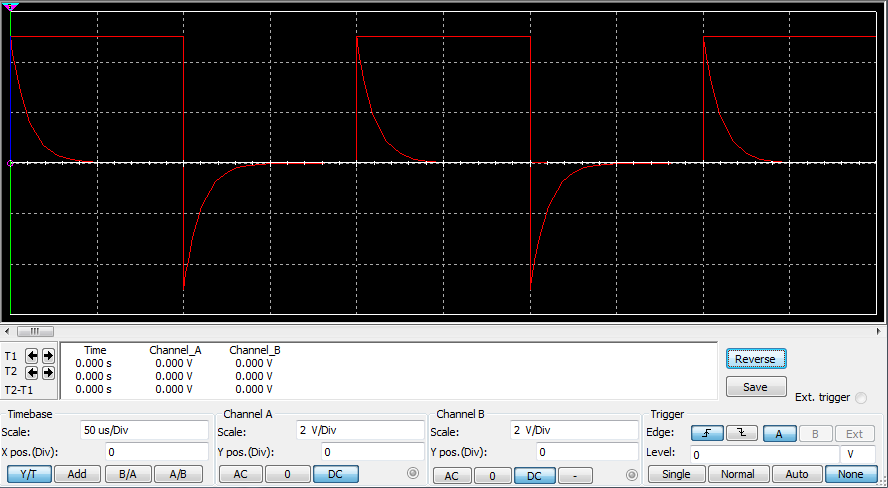
\includegraphics[width=.9\linewidth]{1-a-v_l}
	\caption{RL 회로, $v_L$}
\end{minipage}%
\begin{minipage}{.5\textwidth}
	\centering
	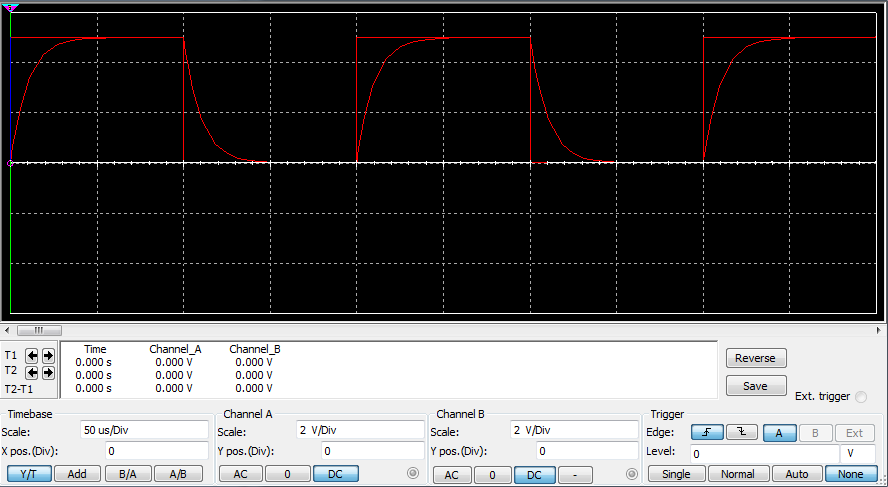
\includegraphics[width=.9\linewidth]{1-a-v_r}
	\caption{RL 회로, $v_R$}
\end{minipage}
\end{figure}

$t=0$일 때에는 전원 전압이 급격하게 커지므로 전류가 급격하게 변하며, 이를 방지하기
위해 인덕터에 큰 전압이 걸린 후 서서히 줄어든다. $t=\frac{T}{2}$인 경우도 마찬가지로
전류가 급격히 줄어드는 것을 방지하기 위해 인덕터에 음의 전원이 걸린다.

저항의 경우, $v_R = v_S - v_L$을 사용해 $v_R$을 구할 수 있다. $v_L$ 그래프를 구형파
에 대하여 상하를 뒤집은 개형을 갖는다.

\subsubsection{RC 회로}
\begin{figure}[H]
\centering
\begin{minipage}{.5\textwidth}
	\centering
	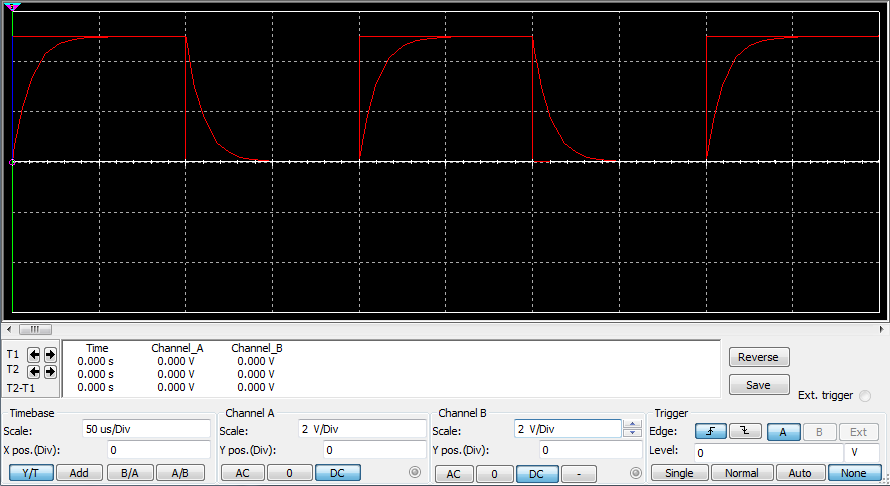
\includegraphics[width=.9\linewidth]{1-b-v_c}
	\caption{RC 회로, $v_C$}
\end{minipage}%
\begin{minipage}{.5\textwidth}
	\centering
	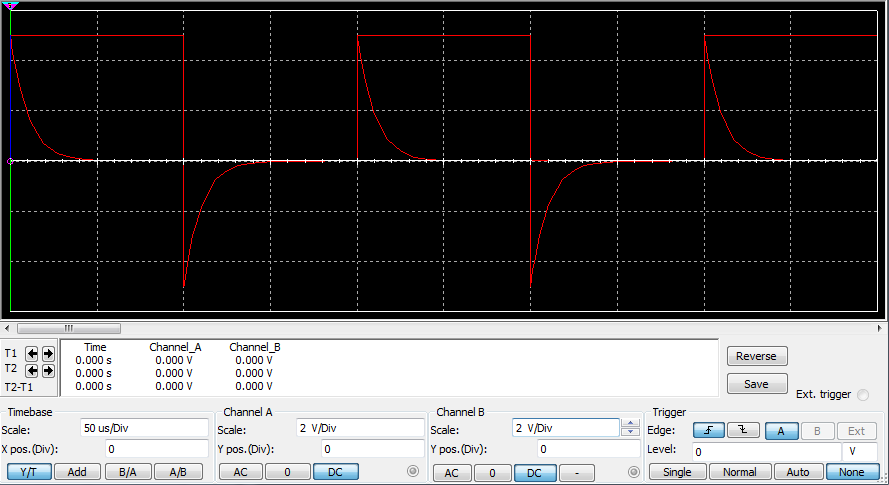
\includegraphics[width=.9\linewidth]{1-b-v_r}
	\caption{RC 회로, $v_R$}
\end{minipage}
\end{figure}

$t=0$일 때에는 전원에 의해 충전이 시작되므로 커패시터의 전압이 지수적으로 상승하여
$v_S$에 점근한다. 반면 $t=\frac{T}{2}$인 경우는 커패시터가 방전되므로 전압이 지수적으로
하강하여 0에 점근한다.

저항의 경우, $v_R = v_S - v_C$을 사용해 $v_R$을 구할 수 있다. $v_C$ 그래프를 구형파
에 대하여 상하를 뒤집은 개형을 갖는다.


\subsection{컴퓨터와 프린터}

\subsubsection{회로 모델}
\begin{figure}[H]
\centering
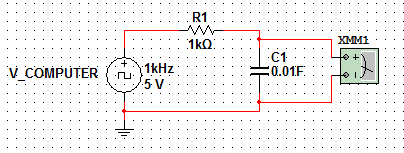
\includegraphics[scale=0.74]{2-a-maybe}
\caption{V\_COMPUTER는 컴퓨터 입력, XMM1은 프린터 출력을 나타냄}
\end{figure}

\subsubsection{연결선 길이}
전압이 1\% 이내가 되는 데 걸리는 시간이 $5\tau$이므로 지연 시간은 $5\tau$와 같다.\\
$5\tau = 5 \cdot RC = 0.5 \cdot 80\times 10^{-12} \cdot l^2 \leq 1ns$이려면\\
\begin{center}
$l \leq \sqrt{1\times 10^{-9} \over {5 \cdot 0.5 \cdot 80\times 10^{-12}}} = 2.236 m$\\
\end{center}
즉, 연결선의 길이가 2.236m 이내이면 주어진 조건을 만족한다.

\subsubsection{회로 구성}
$R=500\Omega$, $C=0.082\mu F$로 설정하면 대략적으로 $l=1000m$일 때 비례상수를 곱하여 구한
저항과 커패시터 값이 된다.
이 때 지연시간 $5\tau = 5 \cdot 500\Omega \cdot 0.082\mu F = 205\mu s$가 된다. Multisim에서 
Oscilloscope 화면으로 대략적으로 측정한 값은 약 $212\mu s$로 오차 3.4\%의 값을 나타내었다.

\begin{figure}[h]
\centering
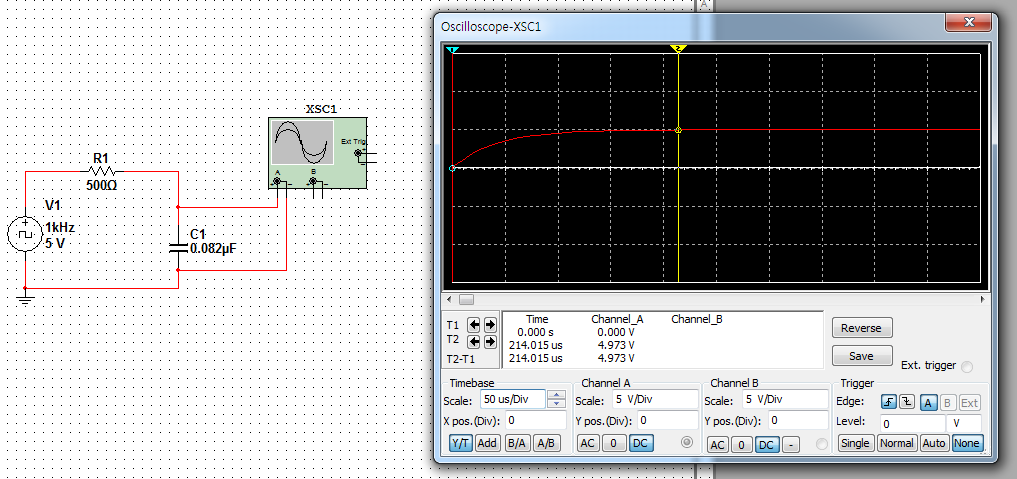
\includegraphics[scale=0.3]{2-b}
\caption{$l=1000m$일 때의 회로 구성}
\end{figure}
\end{document}